\documentclass[a4paper,12pt]{article}
\usepackage[utf8x]{inputenc} %commentaire
\usepackage[francais]{babel} %FR
\usepackage[T1]{fontenc}

\usepackage[pdftex]{graphicx} % img
\usepackage{wrapfig}
\usepackage{float}

\usepackage{algpseudocode}

\usepackage[top=2.5cm, bottom=2.5cm, left=2.5cm, right=2.5cm]{geometry} %Réduire les marges

% Style Page
\pagestyle{myheadings} % entêtes
\sloppy % ne pas faire déborder les lignes dans la marge


\begin{document}
  \section*{Expérience 1}
    \subsection*{Résumé}
      Reproduction et approfondissement des résultats de la première expérience 1 dans l'article 
      \cite{Cleeremans_2007}. 

    
    \subsection*{Pourquoi?}
      Comprendre de quelles manières peuvent émerger des représentations et méta-représentations dans 
      un réseau de neurone connexionniste, en particulier sur des perceptrons multicouches.
    
    
    \subsection*{Architecture}
      \paragraph*{Description}
	Un premier réseau de perceptron multicouche apprend à discrétiser des chiffres représentés
	par 20 neurones d'entrées. Il est composé d'une couche cachée de 5 neurones.
	
	Un second réseau de perceptron multicouche apprend à dupliquer toutes les couches du premier
	réseau en n'ayant que sa couche cachée en entrée.

      \paragraph*{Schéma}
	\begin{center}
	  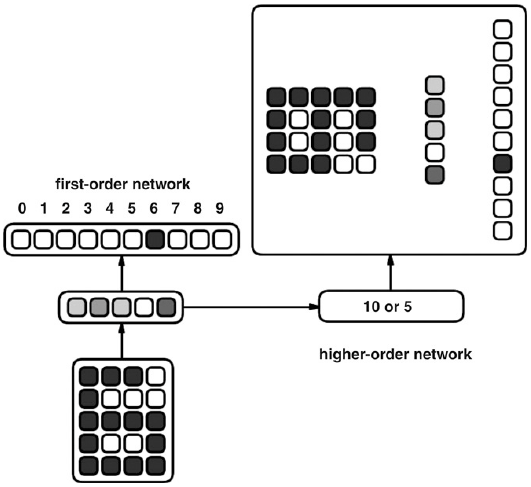
\includegraphics[width=200px]{../cleeremans_2007/digit_reco/digit_reco.png}
	\end{center}
	
      \paragraph*{Paramètres}
        \begin{center}
	  \begin{tabular}{lr}
	    \begin{minipage}{220px}
	      \begin{itemize}
		\item momentum : 0.9 sur les 2 réseau
		\item taux d'apprentissage : 0.1 sur les 2 réseau
		\item 10 chiffres différents présentés
		\item apprentissage 10 (formes) x 1000 (époques)
	      \end{itemize}
	    \end{minipage}
	    &
	    \begin{minipage}{205px}
	      \begin{itemize}
		\item poids initialisés sur [-0.25 ; 0.25]
		\item taux d'apprentissage constant
		\item entrées valent 0 ou 1
		\item sigmoïde à température 1
	      \end{itemize}
	    \end{minipage}
	  \end{tabular}
	\end{center}

    
    \newpage
    \subsection*{Résultats}
      \paragraph*{Principaux}
	\begin{center}
	  \begin{tabular}{lr}
	    \hspace*{-1cm}
	    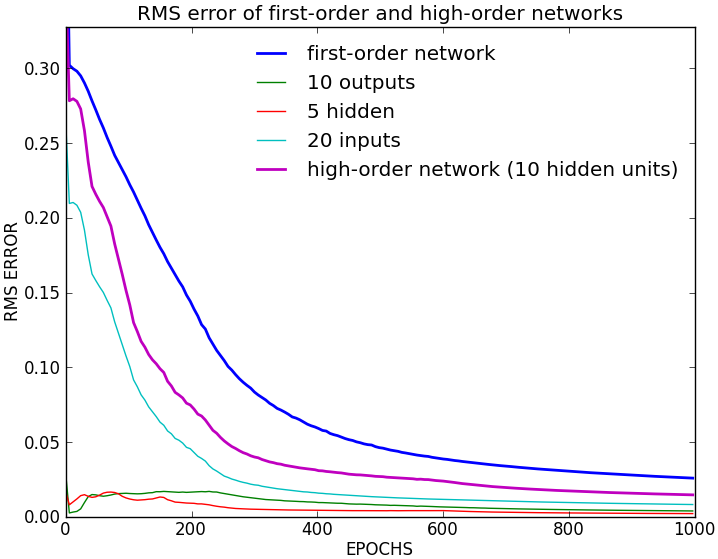
\includegraphics[width=250px]{../cleeremans_2007/digit_reco/rms_ffa.png}
	    &
	    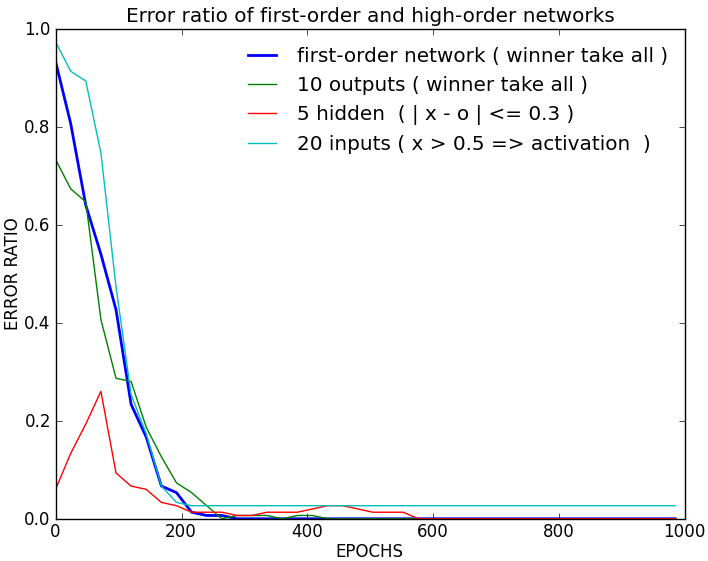
\includegraphics[width=250px]{../cleeremans_2007/digit_reco/err_ffa.png} 
	  \end{tabular}
	\end{center}
	\subparagraph*{Notes}
	  \begin{itemize}
	  \item la courbe violette est la somme des 3 courbes des couches à reproduire.
	  \item 0.3 est le taux de tolérance pour l'erreur sur un neurone
	  \end{itemize}
	  
	\subparagraph*{Conclusion}
	  \begin{itemize}
	    \item la couche cachée et la couche de sortie ne posent aucun problèmes d'apprentissage
	    \item les performances du second réseau dépendent principalement de sa capacité à reproduire les entrées
	  \end{itemize}
	  
	  
	


    \subsection*{Conclusion}
    
    


    \subsection*{Formules}
      RMS proportion pour une époque $e$ est :
      \begin{center}
      \begin{large}
      $ rms\ proportion_{e} = \frac{ rms_{e} = \sqrt{ \frac{1}{n} \sum \limits_{i=1}^{n} 
      ( o_{i,e} - d_{i} )^2 }}{max(rms_{e'}),\ \forall e' \in epochs } $
      \end{large}
      $ with \left\lbrace \begin{array}{lll} n : number\ of\ neurons\ on\ the\ output\ 
      layer\\o_{i,e} : value\ obtained\ for\ the\ i^{th}\ neuron\ at\ the\ e^{th}\ epoch\\d_{i} : 
      value\ desired \ for\ the\ i^{th}\ neuron\end{array} \right.$
      \end{center}
      
    \subsection*{Algorithmes}
      RMS proportion pour une époque $e$ est :
      \begin{center}
      \begin{large}
      $ rms\ proportion_{e} = \frac{ rms_{e} = \sqrt{ \frac{1}{n} \sum \limits_{i=1}^{n} 
      ( o_{i,e} - d_{i} )^2 }}{max(rms_{e'}),\ \forall e' \in epochs } $
      \end{large}
      $ with \left\lbrace \begin{array}{lll} n : number\ of\ neurons\ on\ the\ output\ 
      layer\\o_{i,e} : value\ obtained\ for\ the\ i^{th}\ neuron\ at\ the\ e^{th}\ epoch\\d_{i} : 
      value\ desired \ for\ the\ i^{th}\ neuron\end{array} \right.$
      \end{center}

  \bibliographystyle{../pre-rapport/apalike}
  \bibliography{../pre-rapport/biblio}

\end{document}



